\chapter{Our Proposal: Case Studies}

%We are collaborating with biochemists and pharmacists on several high-impact drug discovery projects.
Our colleagues and collaborators as biochemists and pharmacists are working on several high-impact drug discovery projects. They have done lots of biological assays and succeeded in identifying pharmaceutical and druggable protein targets for certain diseases. They outsource the docking tasks to us, hoping to discover potent and selective inhibitors of certain proteins.

\section{Influenza A Virus H1N1}

%Recent progress in structure-based anti-influenza drug design

Prof. Pang-Chui Shaw and his team from Department of Biochemistry at Chinese University of Hong Kong have studied influenza A virus H1N1 (swine flu) for years. They select the influenza viral nucleoprotein and the influenza A RNA polymerase subunit PA as drug targets, and we assist with structure-based virtual screening.

The influenza viral nucleoprotein, identified as an antiviral target \citep{906}, forms the protein scaffold of the helical genomic ribonucleoprotein complexes, and interacts with the viral RNA polymerase to promote viral RNA replication. Oligomerization of the nucleoprotein is mediated by a flexible tail loop that is inserted into the body domain of a neighbouring molecule and makes extensive interactions through intermolecular $\beta$-sheets, hydrophobic interactions and salt bridges \citep{1140} (Figure \ref{Case:InfluenzaNucleoprotein}, reprinted from \citep{1140}). The displacement of the tail loop from its binding pocket causes significant structural rearrangements in nucleoprotein. Chemical compounds which competitively displace the tail loop from its binding pocket would interfere with viral genome replication, and therefore serve as promising compounds for anti-influenza drug development \citep{1140}.

\begin{figure}
\centering
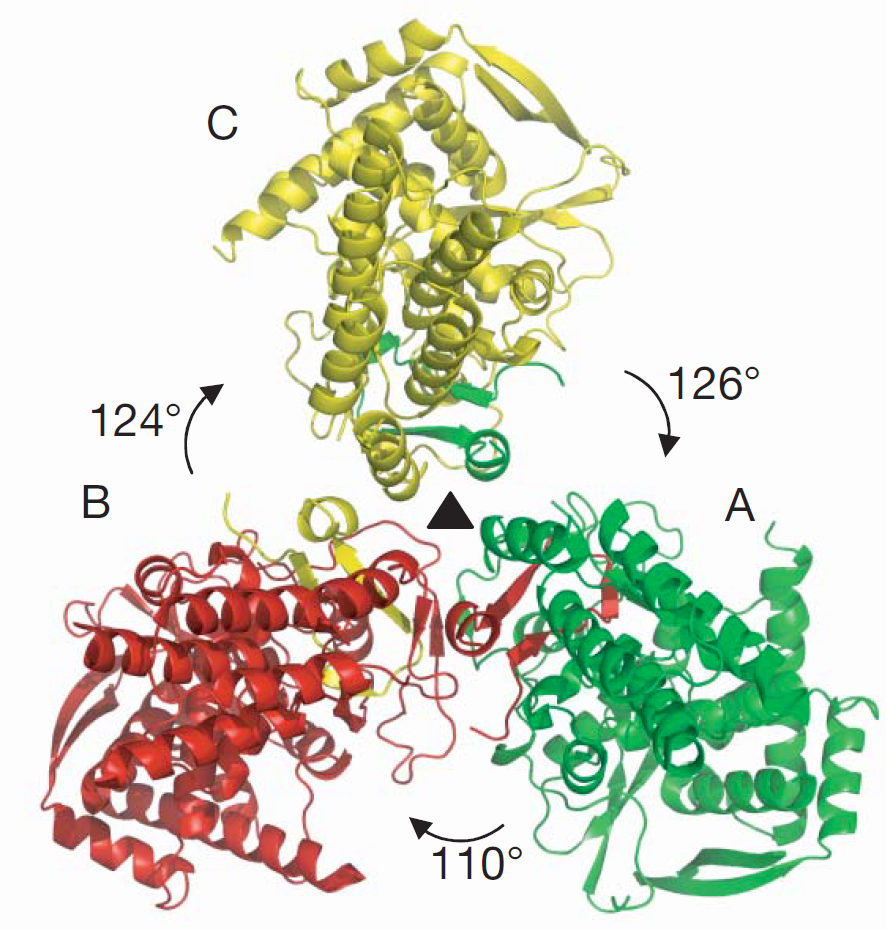
\includegraphics[width=\linewidth]{Case/InfluenzaNucleoprotein.png}
\caption{Nucleoprotein trimer viewed along the NCS (Non-Crystallographic Symmetry) three-fold axis, with three subunits shown in different colors. The rotation angles that relate the three subunits are marked. Figure reprinted from \citep{1140}.}
\label{Case:InfluenzaNucleoprotein}
\end{figure}

The influenza A RNA polymerase is a heterotrimer composed of three subunits, namely PA, PB1 and PB2. It binds the conserved 3' and 5' ends of each of the 8 single-stranded RNA segments in the influenza A virus genome. All the three subunits are required for both transcription and replication. PA is involved in assembly of the functional complex, cap binding and vRNA (virion RNA) promoter binding. PB1 carries the polymerase active site. PB2 includes the capped-RNA recognition domain. On one hand, the carboxy-terminal domain of PA forms a deep and highly hydrophobic groove into which the amino-terminal residues of PB1 can fit by forming a helix and interact through an array of hydrogen bonds and hydrophobic contacts \citep{1141} (Figure \ref{Case:InfluenzaPAPB1}, reprinted from \citep{1141}). The loss of PA abolishes RNA polymerase activity and viral replication. PA and its interface with PB1 are therefore potential drug targets \citep{1141}. On the other hand, PB2 binds the 5' cap of host pre-mRNAs, which are cleaved after 10-13 nucleotides by the endonucleolytic activity of PB1.

\begin{figure}
\centering
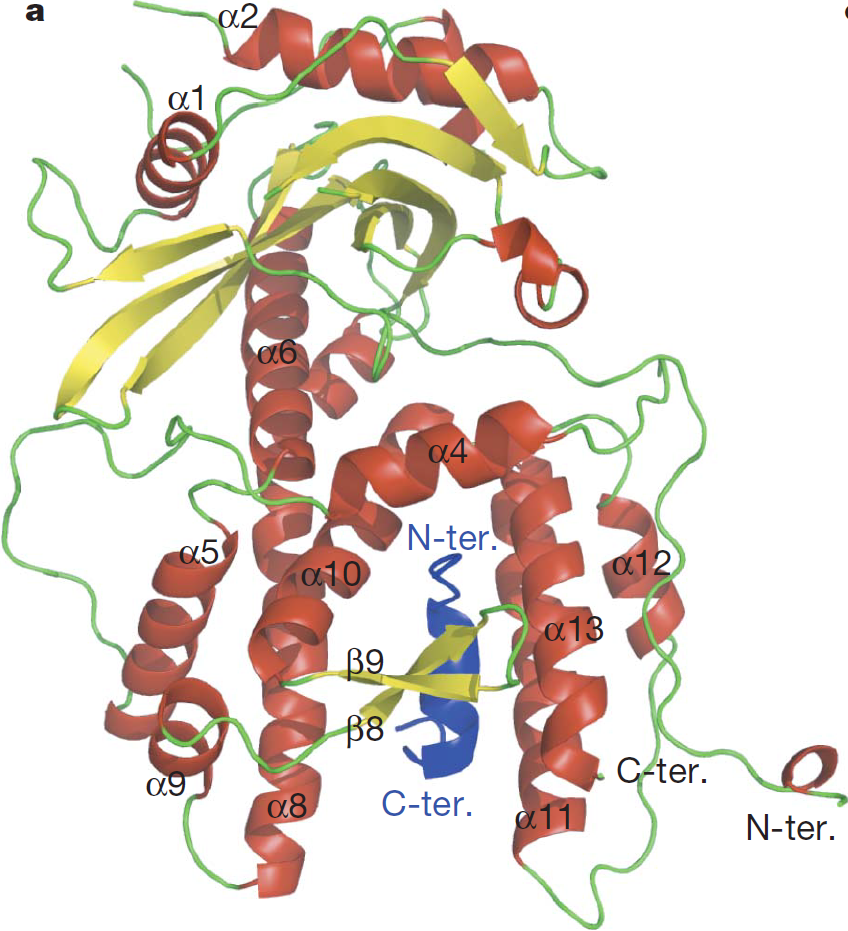
\includegraphics[width=\linewidth]{Case/InfluenzaPAPB1.png}
\caption{Crystal structure of the C-terminal domain of PA bound to the N-terminal peptide of PB1, colored dark blue. Figure reprinted from \citep{1141}.}
\label{Case:InfluenzaPAPB1}
\end{figure}

\begin{figure}
\centering
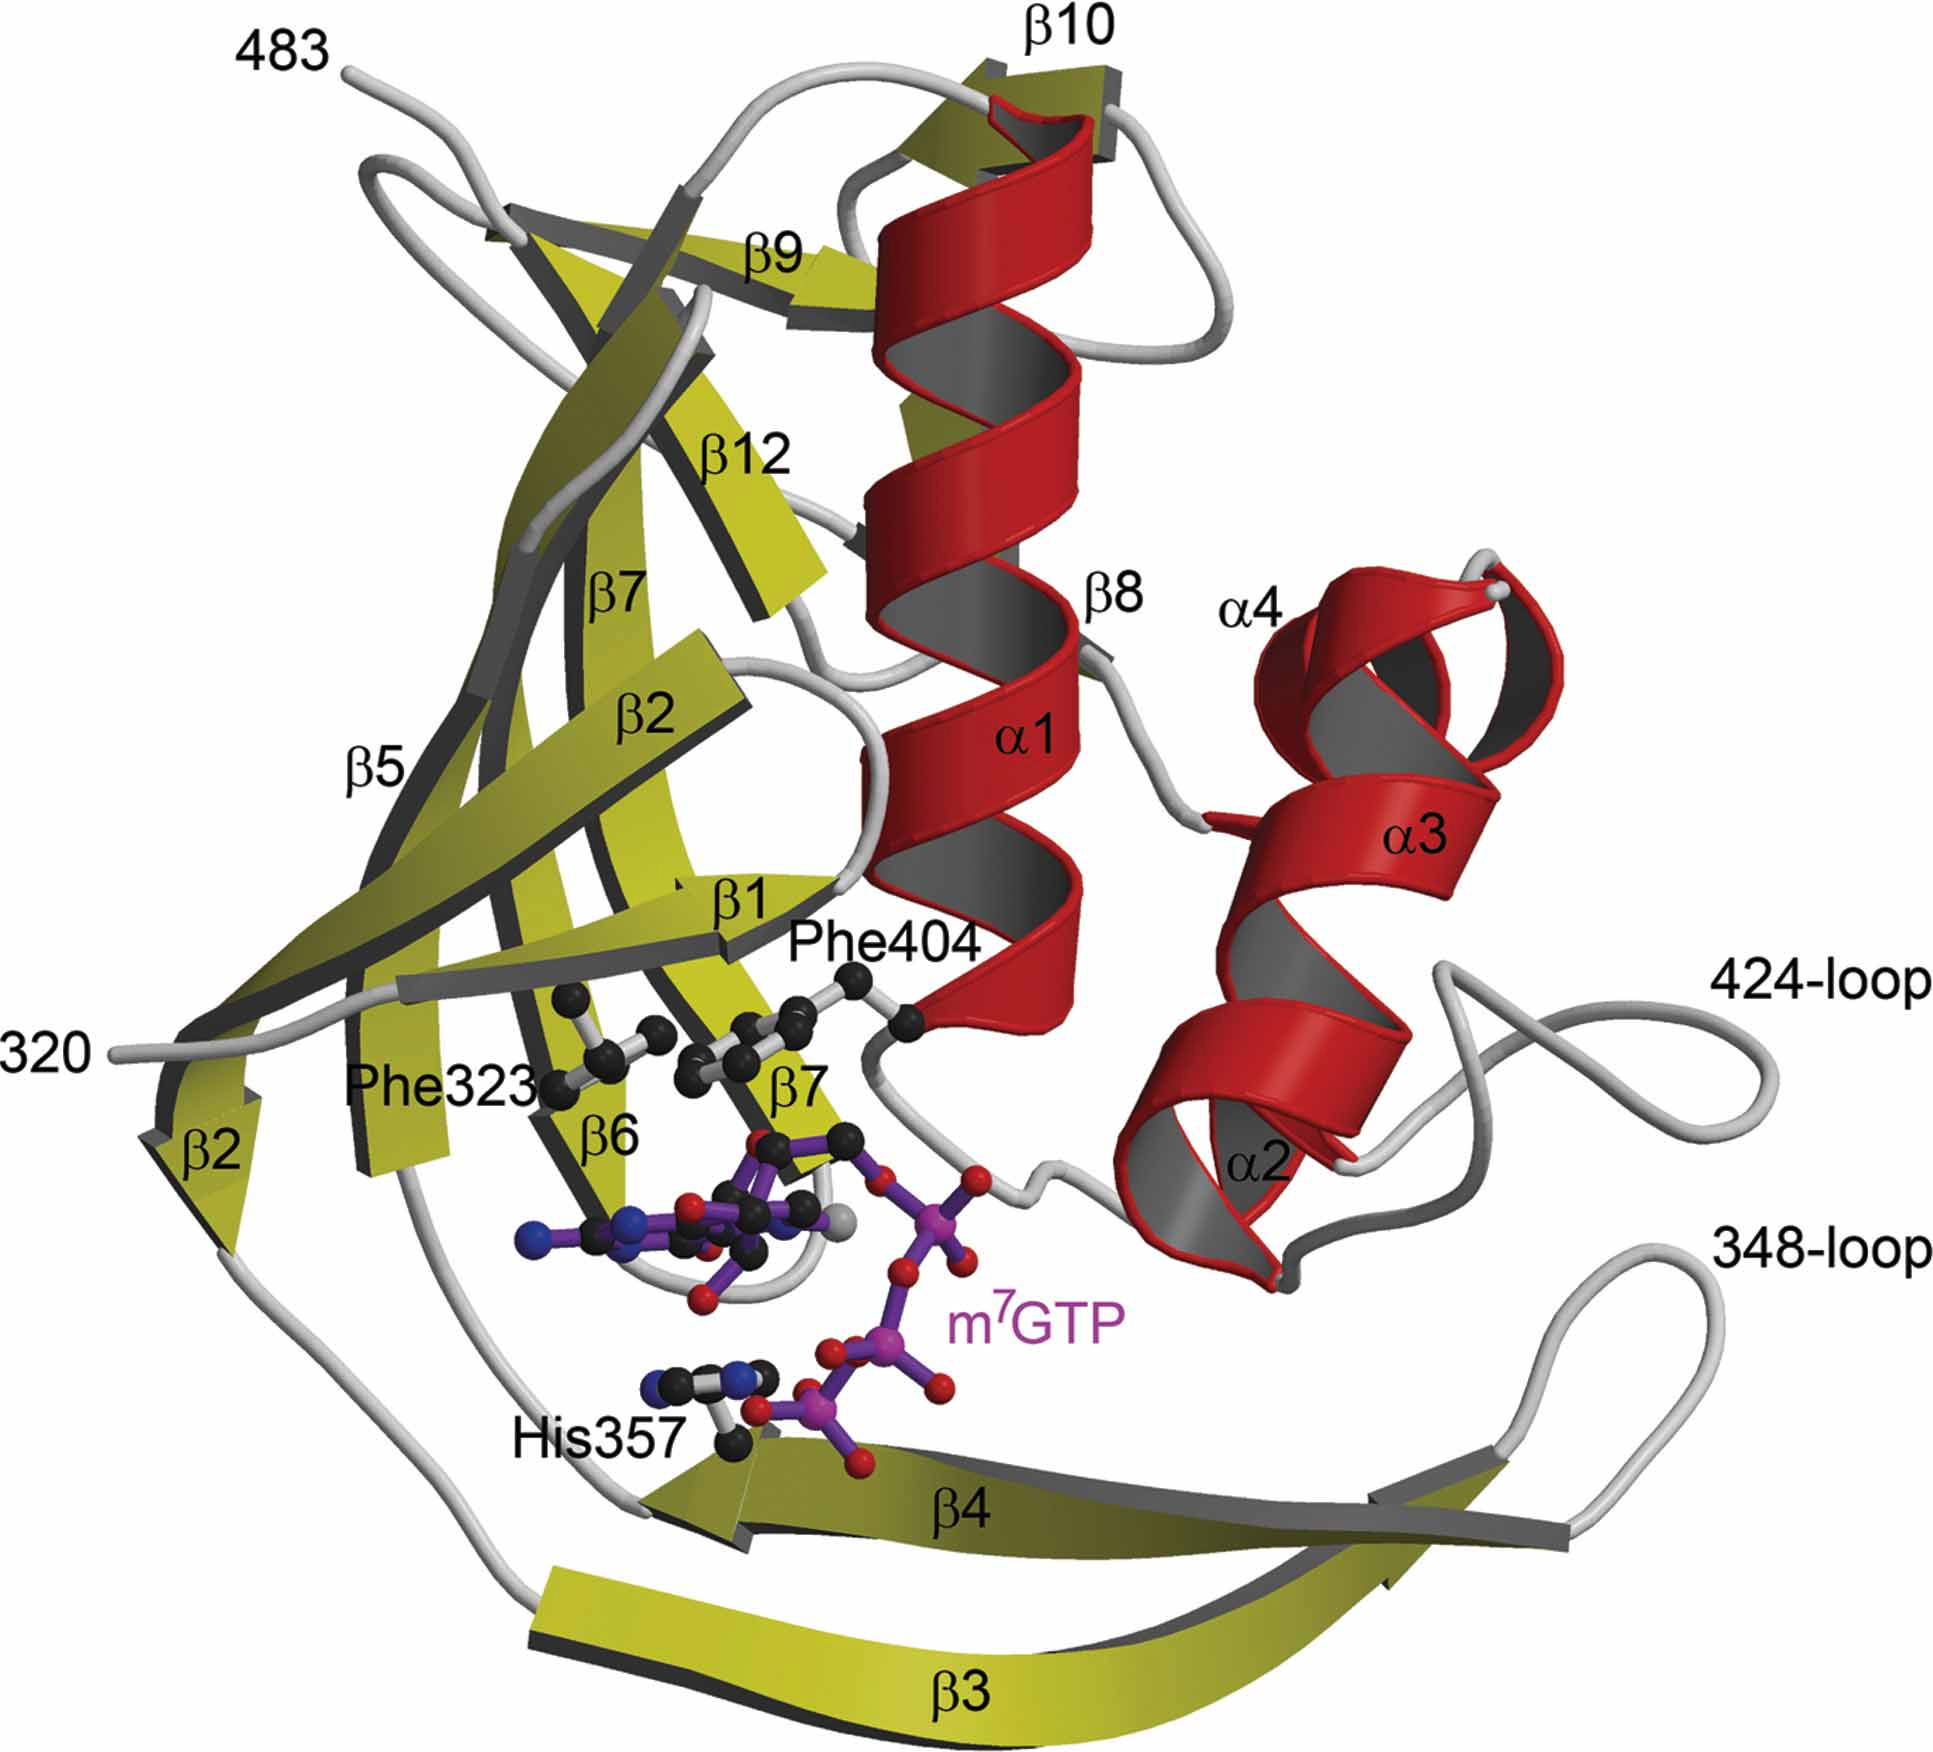
\includegraphics[width=\linewidth]{Case/InfluenzaPB2.png}
\caption{Ribbon diagram of the structure of the PB2 cap binding domain (amino acids 318 to 483) in complex with m\textsuperscript{7}GTP. Figure reprinted from \citep{1192}.}
\label{Case:InfluenzaPB2}
\end{figure}

We are collaborating with Prof. Shaw's team on identifying inhibitors of influenza A H1N1. We obtained the X-ray crystal structures of influenza viral nucleoprotein with PDB ID 2IQH \citep{1140}, influenza A RNA polymerase subunits PA-PB1 complex with PDB ID 2ZNL \citep{1141}, and subunit PB2 in complex with m\textsuperscript{7}GTP with PDB ID 2VQZ \citep{1192}. For the nucleoprotein, we removed chains B and C and only retained chain A. For the PA-PB1 complex, we removed PB1 and only retained PA. For the PB2-m\textsuperscript{7}GTP complex, we removed PB2 chains B, D, E, F and m\textsuperscript{7}GTP and only retained PB2 chain A. Using idock 1.5 with a fine grid map granularity of 0.08\AA, we docked 7,220,835 ZINC \citep{532} clean ligands against nucleoprotein chain A and docked 73,648 ZINC clean ligands against PA. All the ligands are free of yuck compounds and have a molecular weight of at least 350g/mol. The docking took us 5 months. Figures \ref{Case:2IQH-ZINC20464531} and \ref{Case:2IQH-ZINC33733935} depict the interactions between influenza viral nucleoprotein chain A and two high-rank ligands. Figures \ref{Case:2ZNL-ZINC17206951} and \ref{Case:2ZNL-ZINC40879809} depict the interactions between influenza A RNA polymerase subunit PA and two high-rank ligands. Later on we developed idock 1.6 and used it to dock xxx ligands with vendor information available. Such precious experience builds us strong confidence to subsequently work on other influenza A subtypes like H5N1 (bird flu).

\begin{figure}
\centering
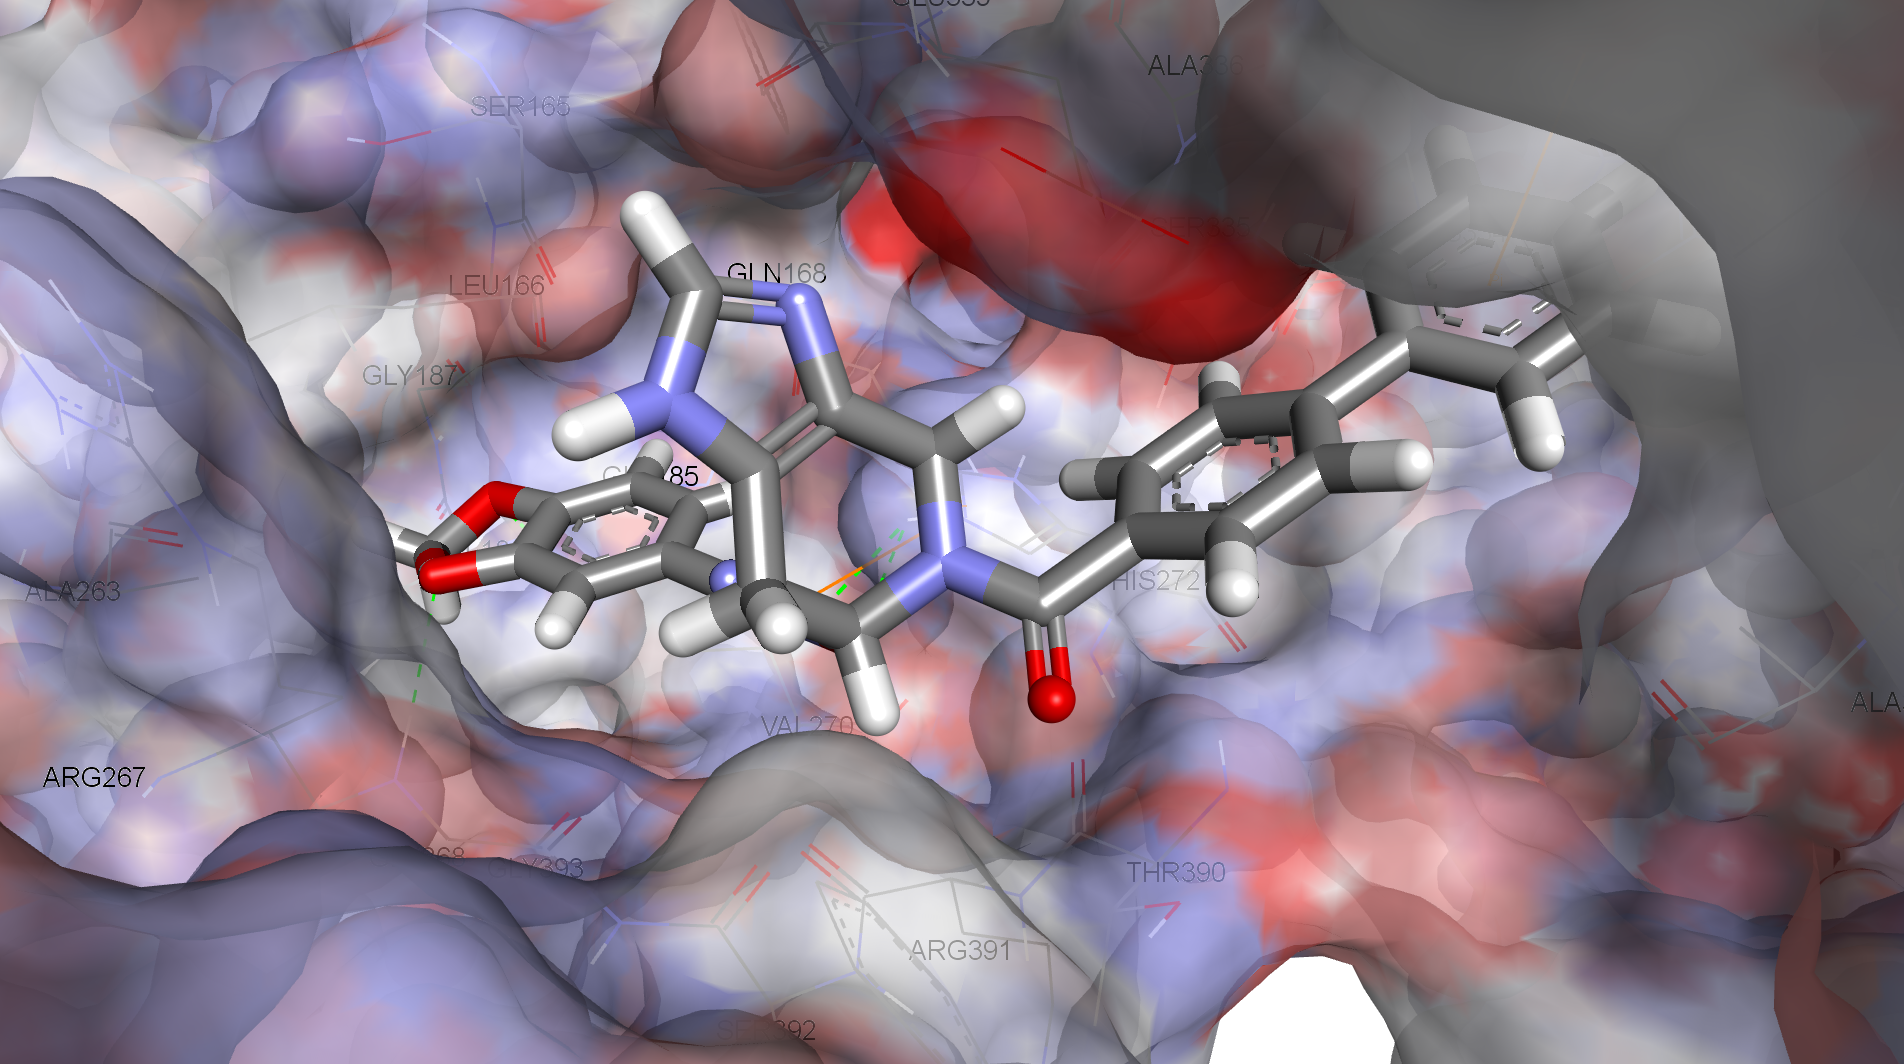
\includegraphics[width=\linewidth]{Case/2IQH-ZINC20464531.png}
\caption{Influenza viral nucleoprotein chain A in complex of ZINC20464531, which forms 4 hydrogen bonds with VAL186, GLY268 and HIS272, Pi-Pi interactions with TRP330, and Pi-Cation interaction with HIS272 and ARG389.}
\label{Case:2IQH-ZINC20464531}
\end{figure}

\begin{figure}
\centering
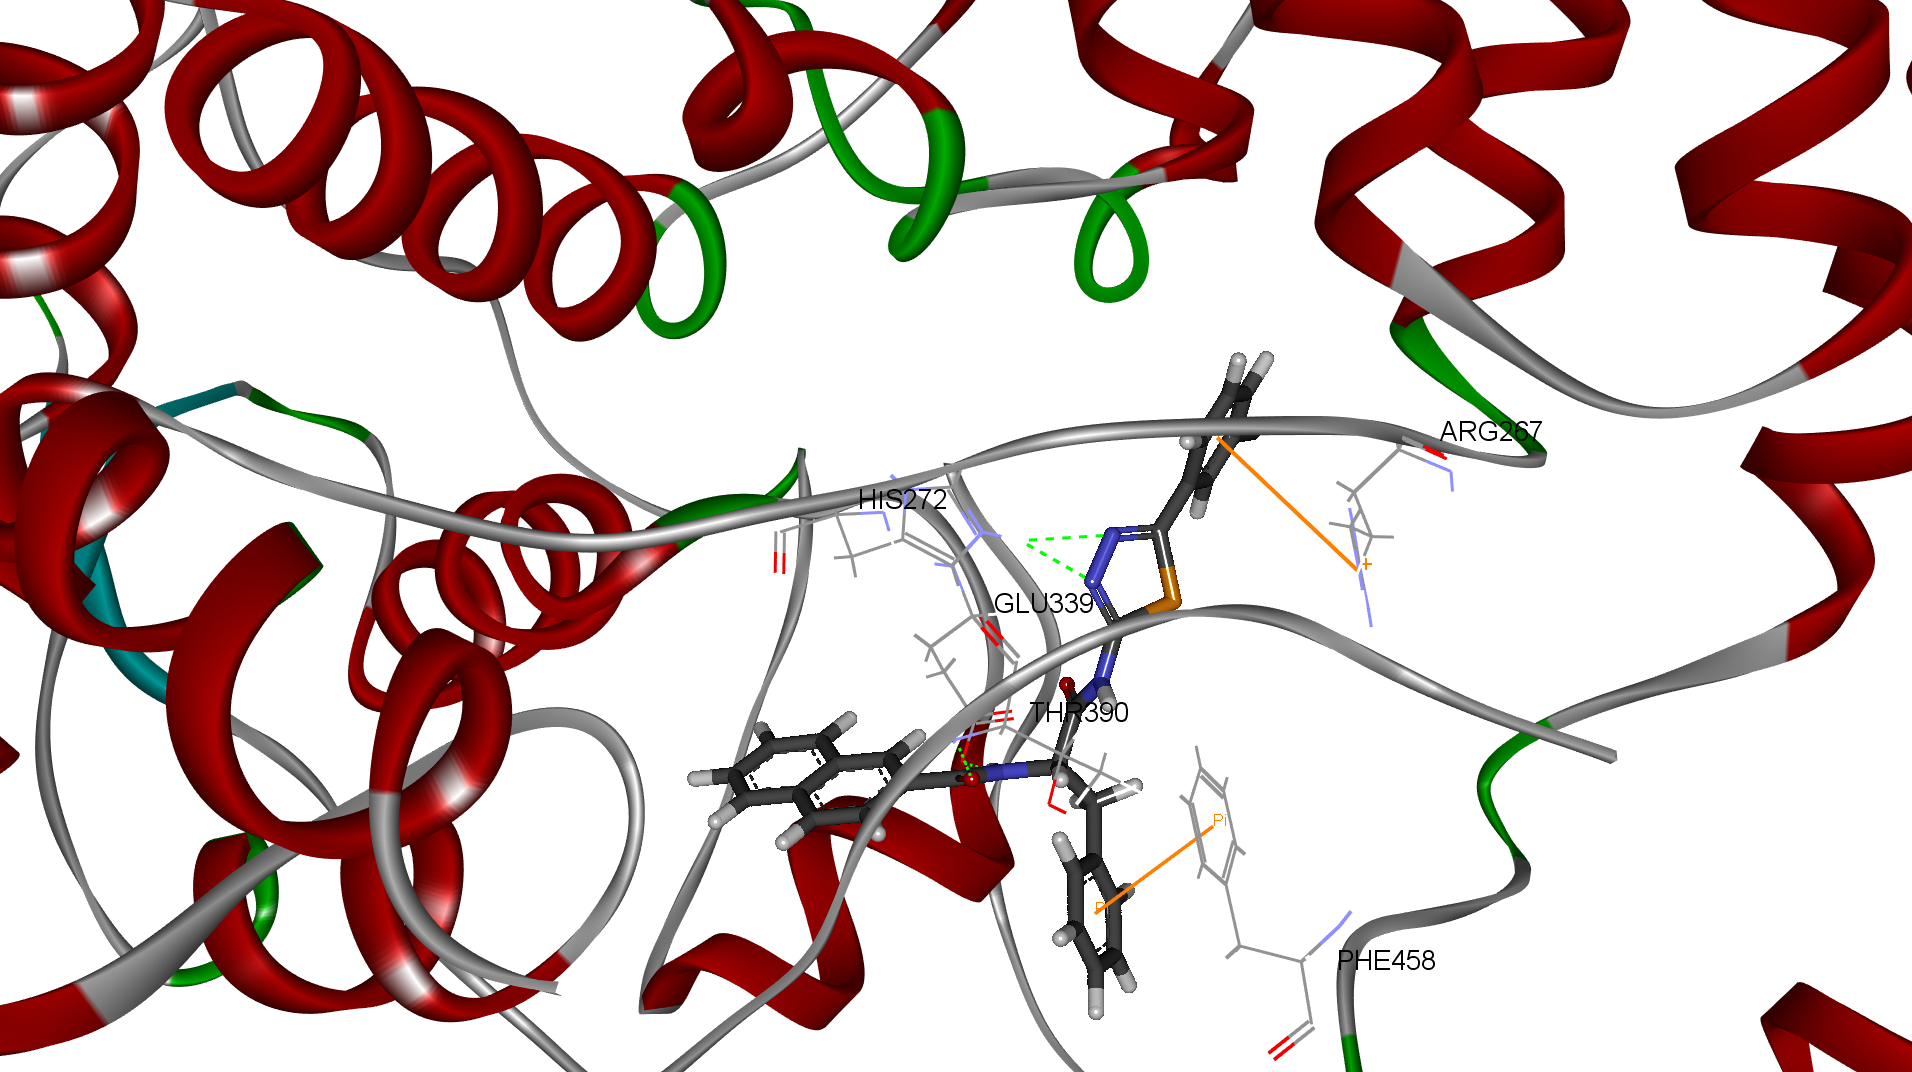
\includegraphics[width=\linewidth]{Case/2IQH-ZINC33733935.png}
\caption{Influenza viral nucleoprotein chain A in complex with ZINC33733935, which forms 2 hydrogen bonds with HIS272 and THR390, Pi-Pi interactions with PHE458, and Pi-Cation interaction with HIS272.}
\label{Case:2IQH-ZINC33733935}
\end{figure}

\begin{figure}
\centering
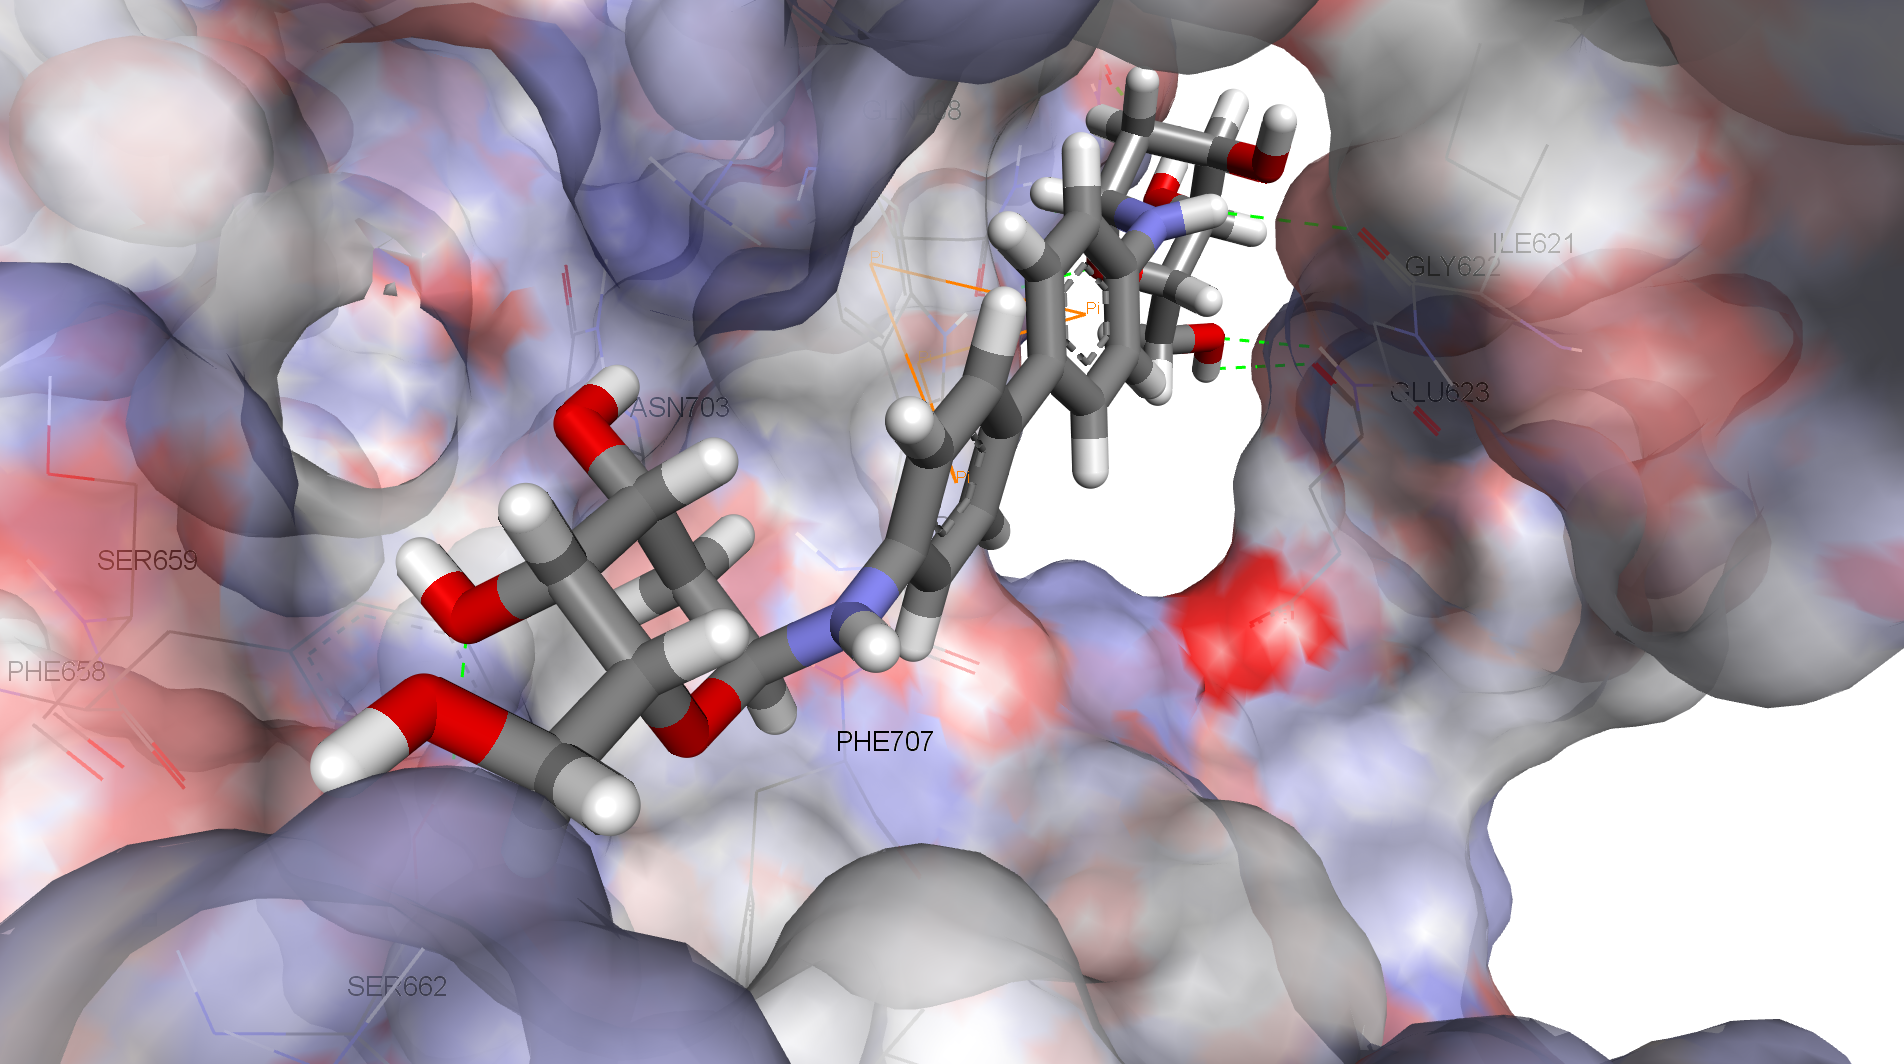
\includegraphics[width=\linewidth]{Case/2ZNL-ZINC17206951.png}
\caption{Influenza A RNA polymerase subunit PA in complex of ZINC17206951, which forms 8 hydrogen bonds with GLN408, ASN412, ILE621, GLU623, SER662 and ASN703, and Pi-Pi interactions with TRP706.}
\label{Case:2ZNL-ZINC17206951}
\end{figure}

\begin{figure}
\centering
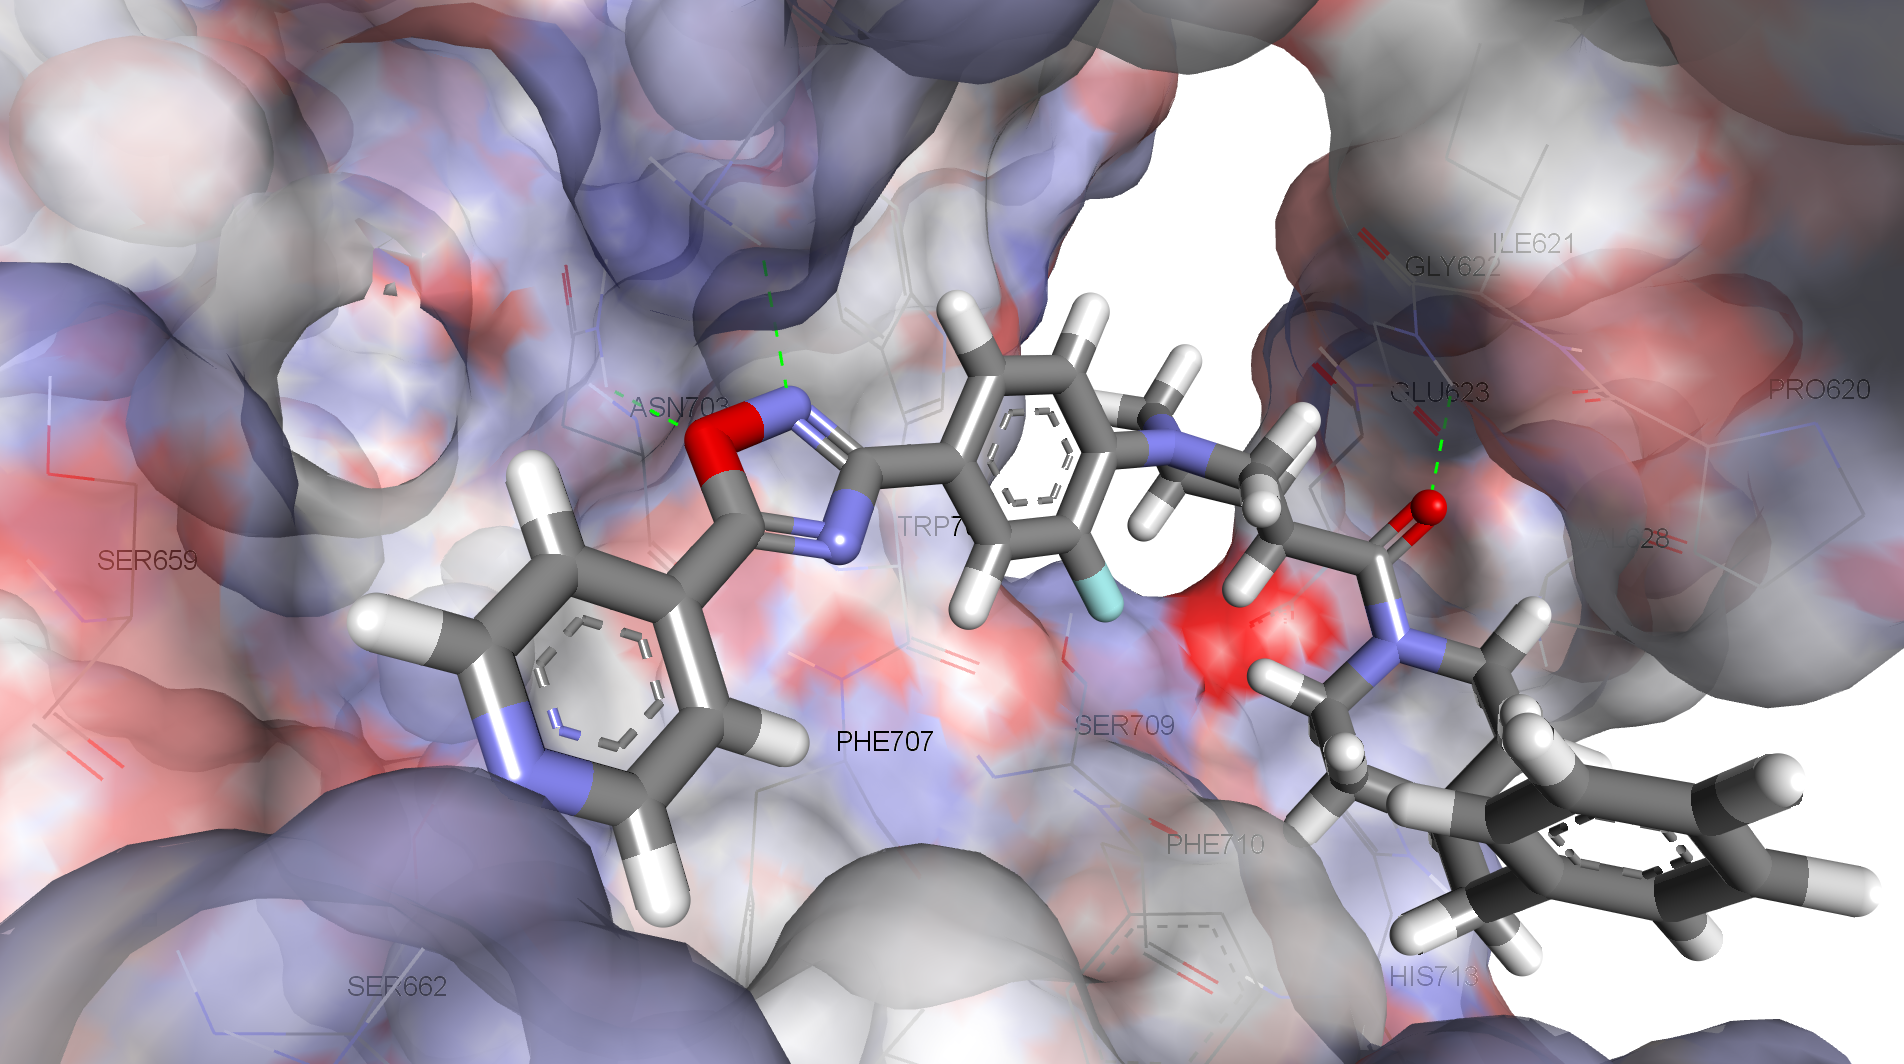
\includegraphics[width=\linewidth]{Case/2ZNL-ZINC40879809.png}
\caption{Influenza A RNA polymerase subunit PA in complex of ZINC40879809, which forms 3 hydrogen bonds with GLY622, LYS643 and ASN703, and Pi-Pi interactions with TRP706.}
\label{Case:2ZNL-ZINC40879809}
\end{figure}

\section{Tumors and Carcinomas}

Prof. Marie Chia-Mi Lin and her team from Department of Surgery at Prince of Wales Hospital investigated the involvement of CCRK (Cell Cycle-Related Kinase) in glioblastoma multiforme carcinogenesis. They analyzed the expression levels of CCRK in 26 glioma patient samples and normal brain, and observed that 1) knock down of CCRK by siRNA (small-interfering RNA) inhibited glioblastoma cell proliferation, 2) suppression of CCRK by shRNA (short hairpin RNA) inhibited glioblastoma tumor growth in nude mice, and 3) CCRK overexpression conferred tumorigenicity to a non-tumorigenic U-138 cell line, and concluded CCRK to be a candidate oncogene in glioblastoma multiforme tumorigenesis \citep{1144}.

Moreover, they examined CCRK expression in a series of ovarian carcinoma tissues by immunohistochemistry, and detected overexpression of CCRK in 53\% of the ovarian carcinomas, and found it positively correlated with patients' clinicopathological characteristics \citep{1145}. They also investigated the role of CCRK in human colorectal cancer carcinogenesis, and found that CCRK protein levels were elevated by more than 1.5-fold in 70\% of colorectal cancer patient samples examined and CCRK was detectable in all seven colorectal cancer cell lines tested \citep{1143}. Suppression of CCRK by siCCRK led to G1 phase cell cycle arrest and reduced cell growth. CCRK is required for the phosphorylation of CDK2 (Cyclin-Dependent Kinase 2) on Thr160 and Rb on Ser795 and the expression of cyclin E \citep{1143}. 

Furthermore, together with Prof. Joseph Jao-Yiu Sung's team, they used genome-wide location and functional analyses to identify CCRK as a direct androgen receptor-regulated gene that drives $\beta$-catenin/T cell factor-dependent hepatocarcinogenesis \citep{1146}. Conversely, knock down of CCRK decreased hepatocellular carcinoma cell growth. CCRK overexpression correlated with the tumor staging and poor overall survival of patients \citep{1146}.

They therefore attempted to seek for CCRK inhibitors for the treatment of cancers and drug resistances. Due to the absence of CCRK structure in the PDB database \citep{540,537}, they utilized Chem3D from the then CambridgeSoft company, now acquired by PerkinElmer, Inc., to build a homologous model of CCRK from CDK2 based on the fact that they share 35\% sequence identity, and performed protein-ligand docking of TCMs (Traditional Chinese Medicines) with AutoDock 3.0.5 and Cerius2 LigandFit, and identified 22-O-Angeloyl theasapogenol B as a potential potent inhibitor that could fit into the deep and narrow active site of their homologous model of CCRK. It was, nevertheless, very difficult to purify the compound from puerh tea.

We are collaborating with Prof. Lin's team on identifying inhibitors of CCRK. We used as receptor the CCRK homologous model (Figure \ref{Case:CCRKHomologousModel}) built by Dr. William Cheung based on the CDK2 template with PDB ID 1HCL \citep{1142} using SWISS-MODEL, a fully automated protein structure homology-modeling server accessible via the ExPASy web server. We concentrated on repurposing approved drugs \citep{944,1023} because developing a drug \textit{de novo} is a laborious and costly endeavor. Using idock 1.5 with a fine grid map granularity of 0.08\AA\ and 512 Monte Carlo tasks, we screened 1,715 FDA-approved drugs via DrugBank and 3,176 FDA-approved drugs via DSSTOX. Figures \ref{Case:1HCL-ZINC03830332} and \ref{Case:1HCL-ZINC03831625} depict the interactions between the CCRK homologous model and two high-rank ligands.

\begin{figure}
\centering
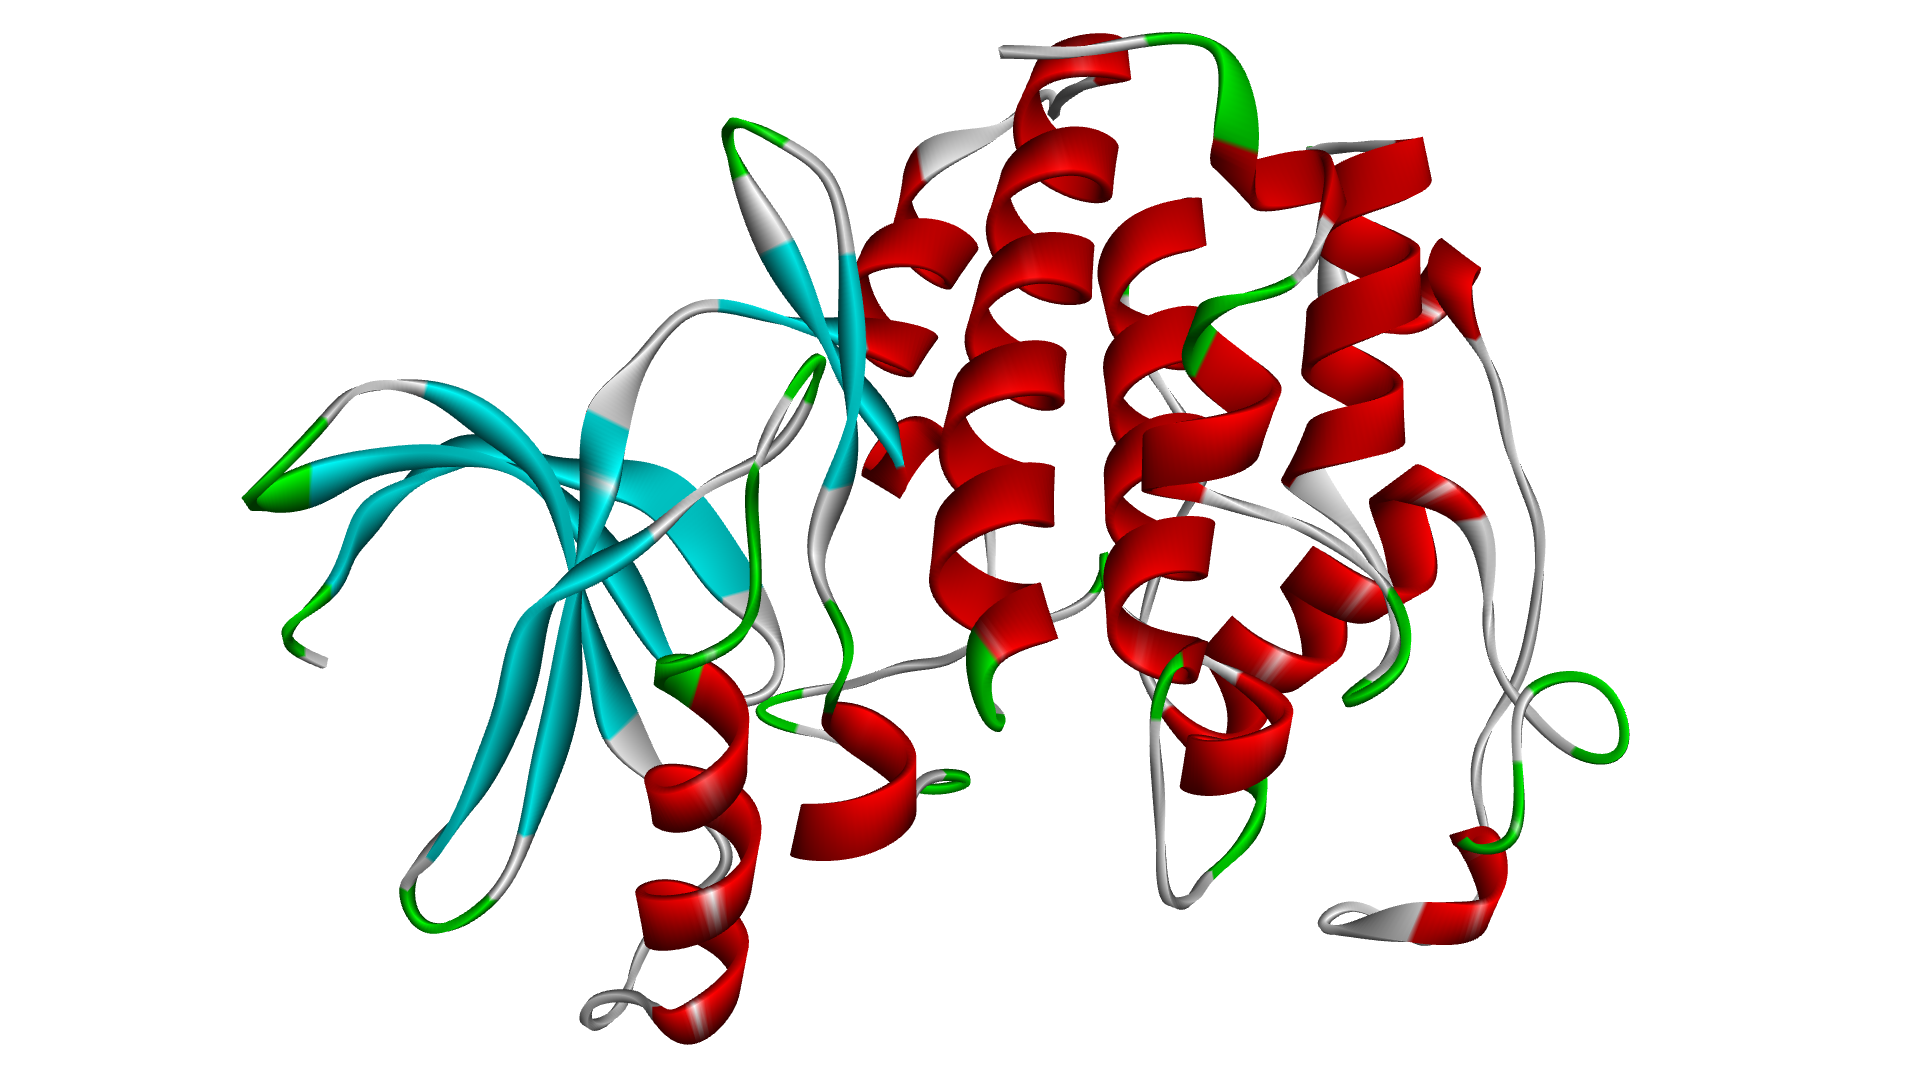
\includegraphics[width=\linewidth]{Case/CCRKHomologousModel.png}
\caption{CCRK homologous model, built by Dr. William Cheung based on the CDK2 template with PDB ID 1HCL \citep{1142} using SWISS-MODEL. The ligand denotes the Ser/Thr protein kinase active site.}
\label{Case:CCRKHomologousModel}
\end{figure}

\begin{figure}
\centering
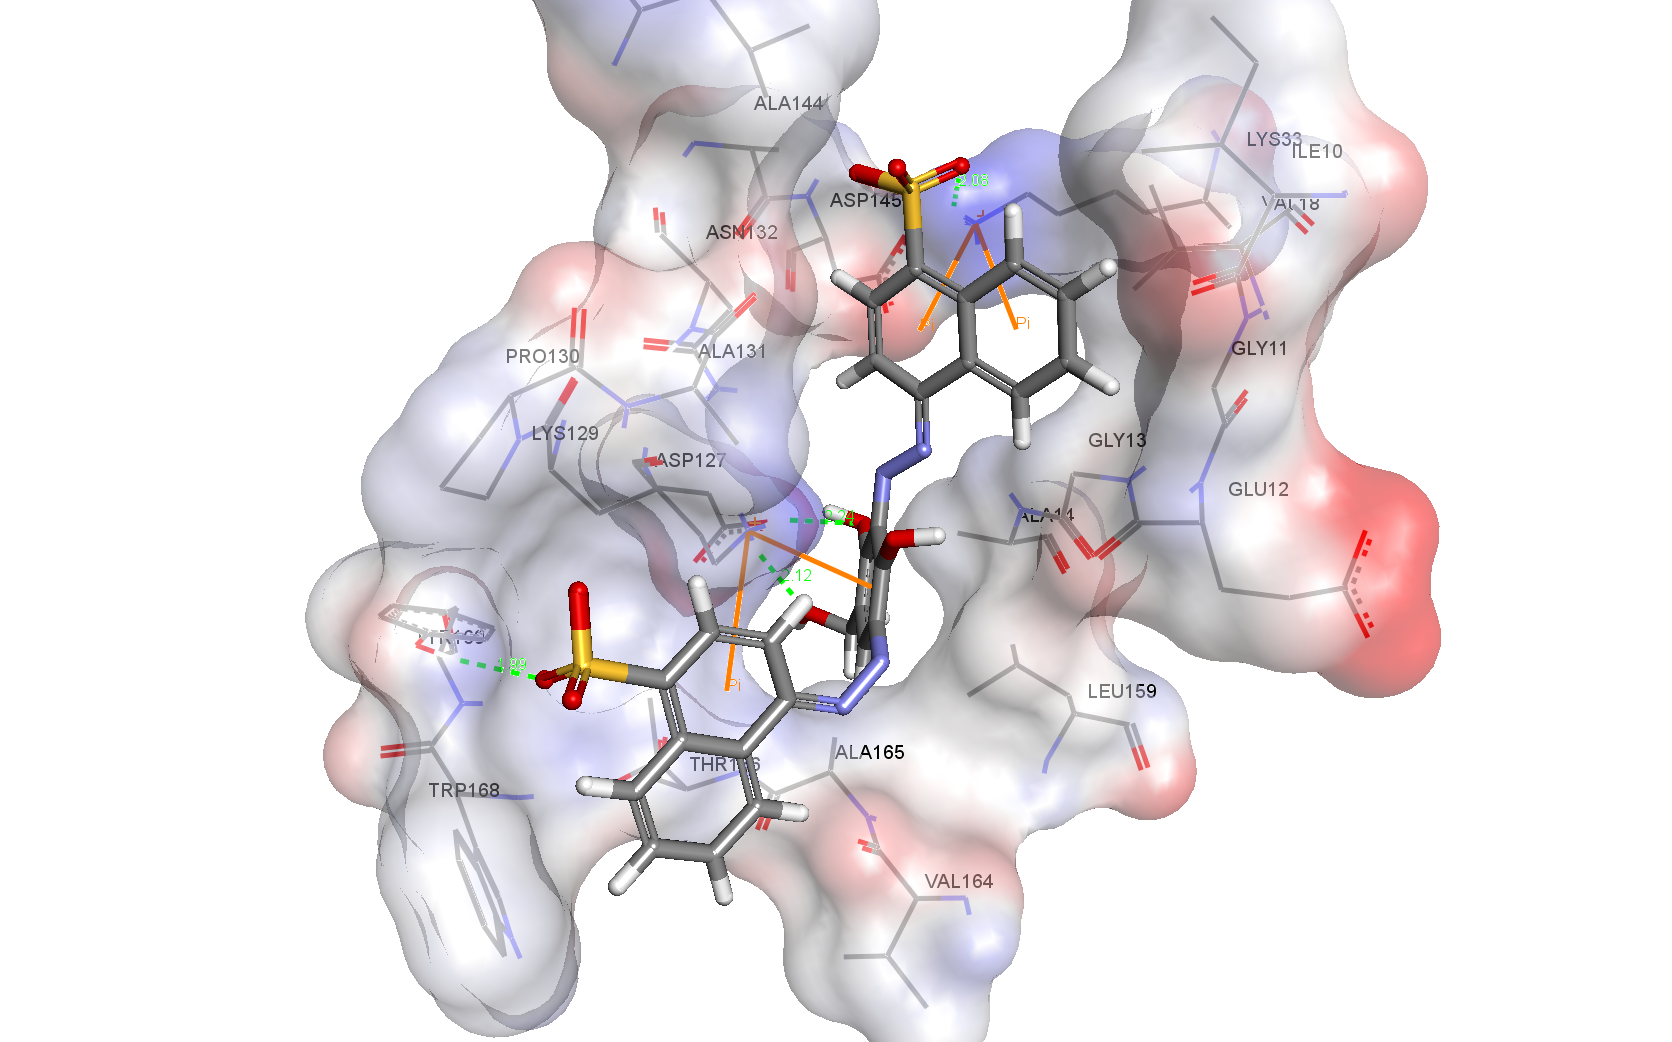
\includegraphics[width=\linewidth]{Case/1HCL-ZINC03830332.png}
\caption{CCRK homologous model in complex of ZINC03830332, which forms 4 hydrogen bonds with LYS33, LYS129 and TYR169, and Pi-Cation interactions with LYS33 and LYS129.}
\label{Case:1HCL-ZINC03830332}
\end{figure}

\begin{figure}
\centering
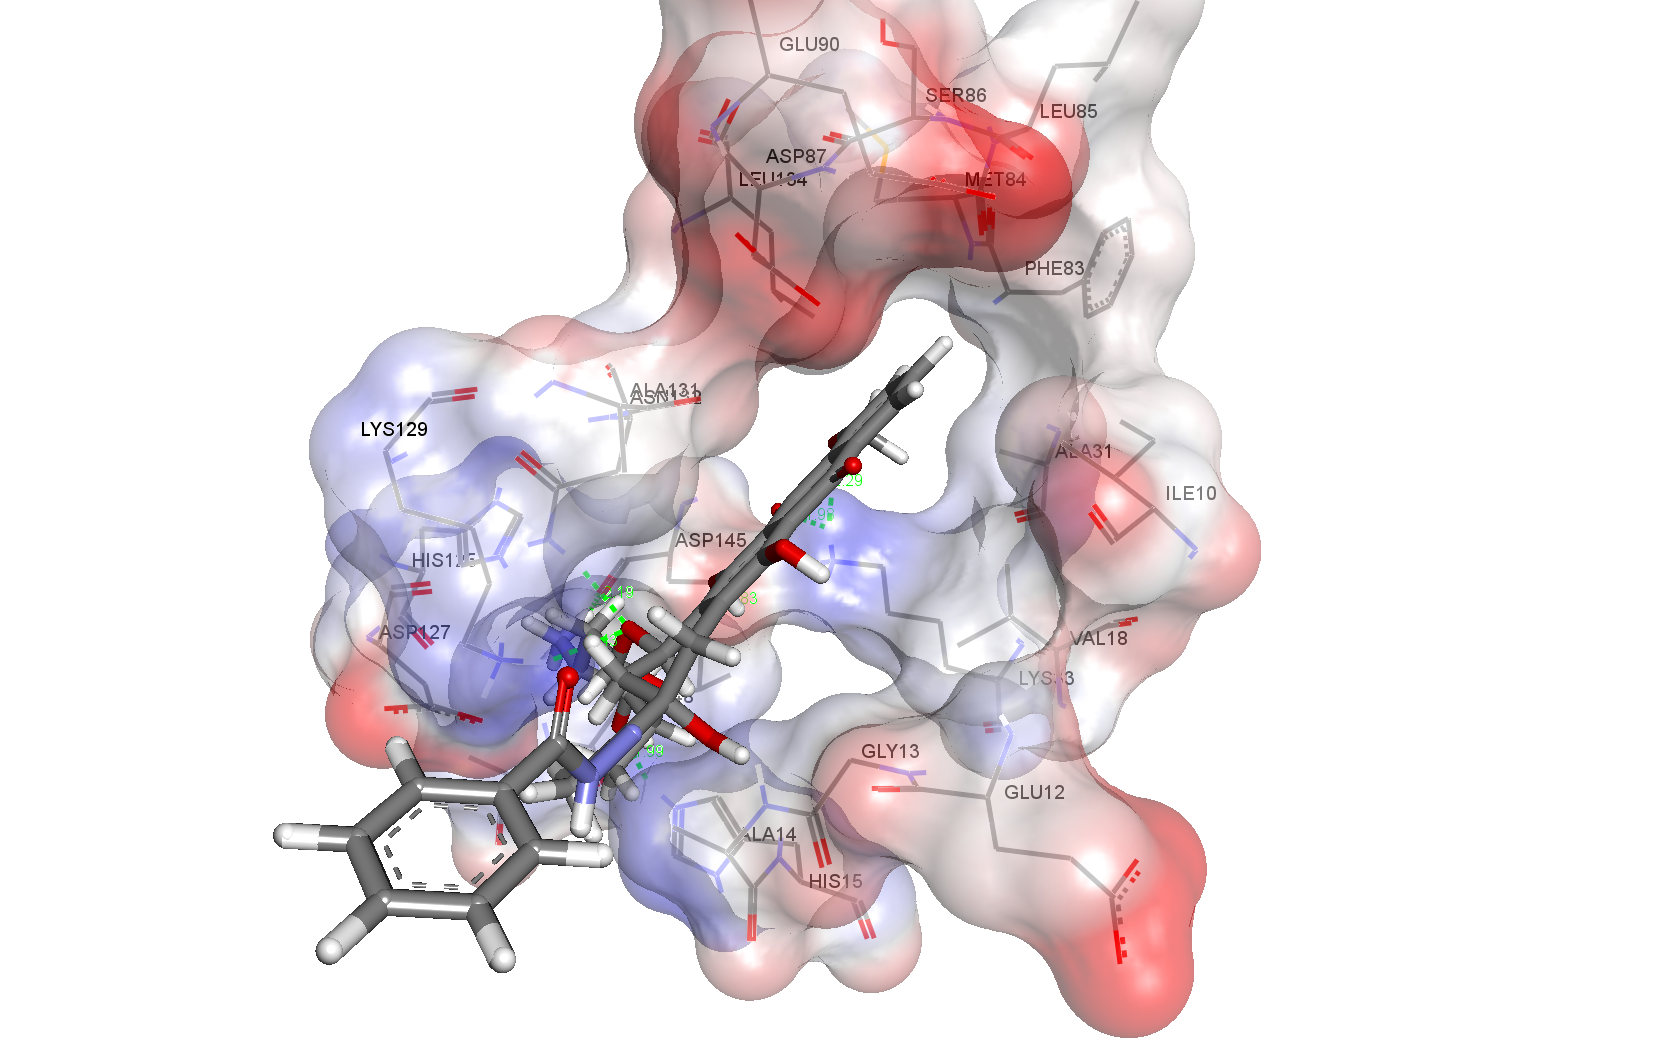
\includegraphics[width=\linewidth]{Case/1HCL-ZINC03831625.png}
\caption{CCRK homologous model in complex of ZINC03831625, which forms 7 hydrogen bonds with HIS15, LYS33, LYS129, ASN132 and ASP145.}
\label{Case:1HCL-ZINC03831625}
\end{figure}

\section{Cancer Stem Cells}

Prof. Hsiang-Fu Kung and Dr. Hong Yao from Stanley Ho Centre for Emerging Infectious Diseases at Chinese University of Hong Kong are seeking specific therapies targeted at CSCs (Cancer Stem Cells) for improvement of survival and quality of life of cancer patients.

CSCs are cancer cells that possess the ability to give rise to all cell types found in a particular cancer sample. As the highly malignant seeds of tumors, CSCs typically comprise 1-5\% of the tumor but give rise to 95-99\% of other tumor cells known as the tumor bulk, and are therefore tumorigenic. While standard therapies, including chemotherapy and radiation, may initially shrink tumors by killing tumor bulk, the failure of these therapies to eradicate CSCs may attribute to treatment failure, tumor relapse and poor survival (Figure \ref{Case:CancerStemCell}).

\begin{figure}
\centering
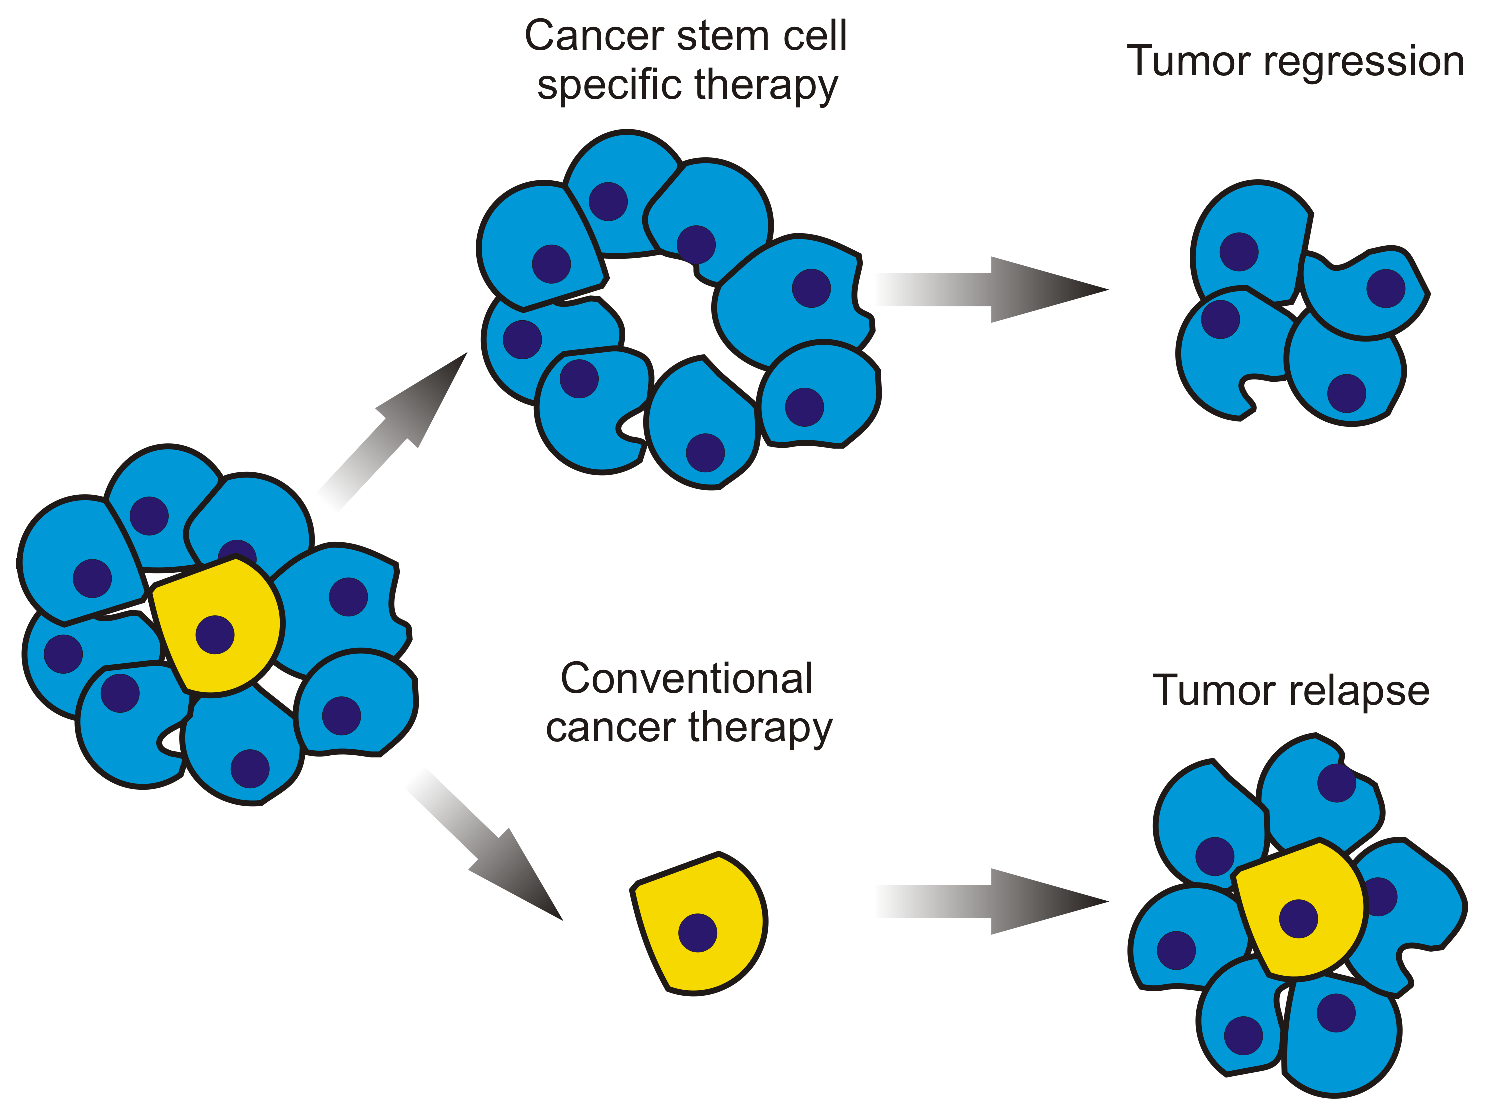
\includegraphics[width=\linewidth]{Case/CancerStemCell.eps}
\caption{CSCs-specific and conventional cancer therapies. Cells in blue are normal cancer cells. Cells in yellow are CSCs. Source: Wikipedia.}
\label{Case:CancerStemCell}
\end{figure}

Salinomycin (Figure \ref{Case:SalinomycinEtoposideAbamectinNigericin}, reprinted from \citep{1147}), a monocarboxylic polyether antibiotic widely used as an anticoccidiosis agent in chicken, was discovered in a chemical screen to selectively kills breast CSCs and reduce the proportion of CSCs by >100-fold relative to paclitaxel, a commonly used breast cancer chemotherapeutic drug. Treatment of mice with salinomycin inhibits mammary tumor growth \textit{in vivo} and induces increased epithelial differentiation of tumor cells \citep{1147}. At the molecular mechanism level, salinomycin specifically inhibits the Wnt/$\beta$-catenin signaling pathway initiated by Wnt1 and selectively induces apoptosis in chronic lymphocytic leukemia cells \citep{1148}.

\begin{figure}
\centering
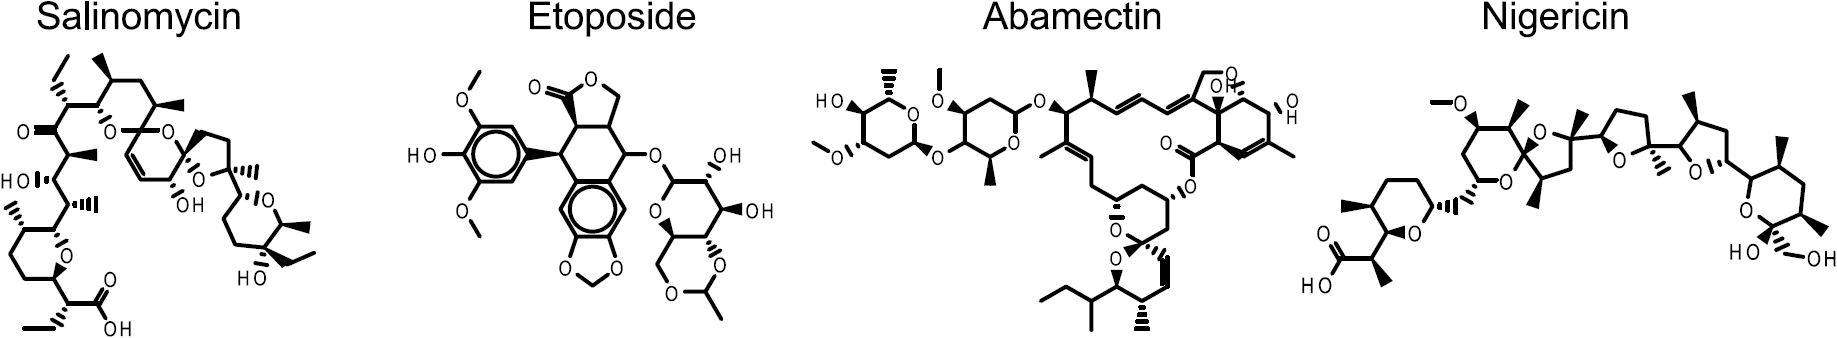
\includegraphics[width=\linewidth]{Case/SalinomycinEtoposideAbamectinNigericin.png}
\caption{Chemical structures of salinomycin, etoposide, abamectin, and nigericin, compounds that exhibit selective toxicity for mesenchymally transdifferentiated epithelial cells. Figure reprinted from \citep{1147}.}
\label{Case:SalinomycinEtoposideAbamectinNigericin}
\end{figure}

We are collaborating with Prof. Kung's team on identifying inhibitors of CSCs. We confirm the Wnt protein as a potential pharmaceutical target of therapeutic interest. The major obstacle right now is the lack of resolved or homologous structures of Wnt. We can neither find a Wnt structure from the PDB database \citep{540,537}, nor predict its structure from known templates (Figure \ref{Case:WntHomologyModeling}). Although the 1JLT template shares 42\% sequence identity with Wnt, it only covers a small range of amino acids from 319 to 360. Ironically, the 1GTE template covers amino acids 13 to 354, but the sequence identity is as low as 14\%, far from sufficient for an accurate homologous model. In reality, we tried five online homology modeling servers, namely ModWeb, M4T, SWISS-MODEL, I-TASSER, and HHpred, but most of them simply refused our job just because of the surprisingly low sequence identity percentage. Therefore, rather than Wnt, one possible way to go is to explore other CSCs-associated signaling pathways such as Bmi-1, Shh, Notch, \textit{Hox} family, Pten, etc.

\begin{figure}
\centering
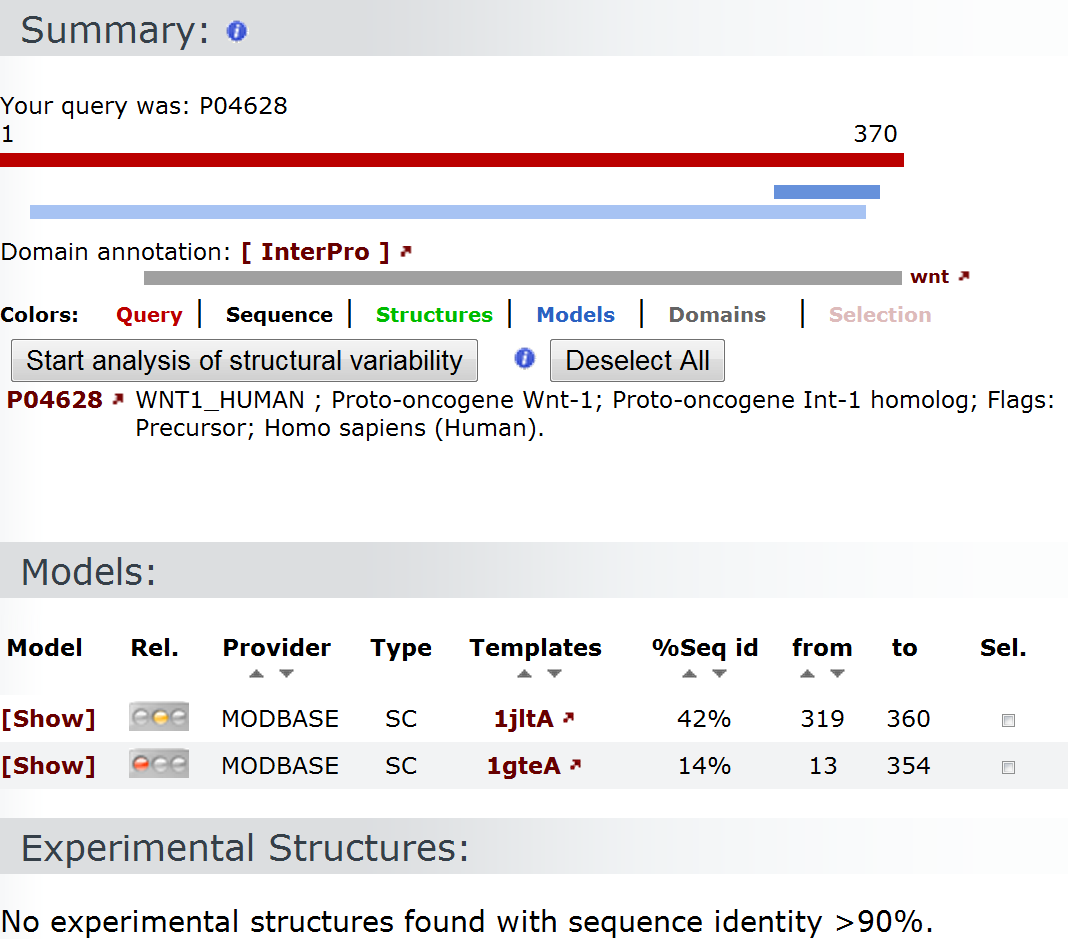
\includegraphics[width=\linewidth]{Case/WntHomologyModeling.png}
\caption{Proto-oncogene Wnt-1 of UniProt ID P04628 shares sequence identity with merely two templates, 1JLT chain A and 1GTE chain A. Source: The Protein Model Portal.}
\label{Case:WntHomologyModeling}
\end{figure}

\chapterend
